\pagestyle{empty}
\begin{center}
  \vspace*{3cm}
  
\begin{tikzpicture}[y = -1cm, scale = .40]
    \draw (0, 0) -- (4, 0) -- (4, 4) -- (5, 4) -- (5, 0) -- (10, 0) --
          (10, 5) -- (9, 5) -- (9, 1) -- (8, 1) -- (8, 5) -- (7, 5) --
    (7, 1) -- (6, 1) -- (6, 5) -- (3, 5) -- (3, 1) -- (2, 1) --
    (2, 5) -- (1, 5) -- (1, 1) -- (0, 1) -- cycle
    %[line width = 0pt, draw = white, fill = tumblue];
    [fill = black, line width = 0pt, draw = white];
  \end{tikzpicture}

  \vspace*{0.5cm}
  {\huge \textsc{Department of Informatics}}\\
  \vspace{0.25cm}
  {\Large \textsc{Technical University of Munich}} \\
  \vspace*{2cm}
  {\large Master's Thesis in Informatics} \\
  \vspace*{2cm}
  {\huge \textbf{Profiling GPU Shaders for Profile-Guided Optimizations} \\}
  \vspace*{2cm}
  {\large Sebastian Neubauer }\\
  \vspace*{2cm}
  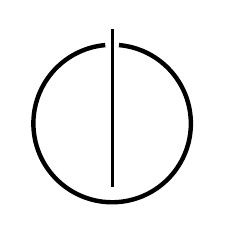
\begin{tikzpicture}
    \draw (0, 0) arc (95:445:1cm) [ultra thick, draw = black];
    \draw (0.09, 0.2) -- (0.09, -1.8) [very thick, draw = black];
  \end{tikzpicture}
  \vfill
  %\begin{center}
  %  \footnotesize Version 1.0 (\today)
  %\end{center}
\end{center}
